\subsection{When}\label{when}
\begin{center}

\textit{Quali sono le ultime novità? Quando è stato aggiornato l'ultima volta?}

\end{center}
\begin{flushleft}
Il sito non permette di raggiungere agevolmente tali contenuti nella homepage, 
questi possono essere visualizzati solamente scrollando fino all'ultima pagina. Alternativamente è possibile selezionare la sezione \textit{Blog}
 presente nel menù di navigazione.
    \begin{figure}[ht]
    \centering
    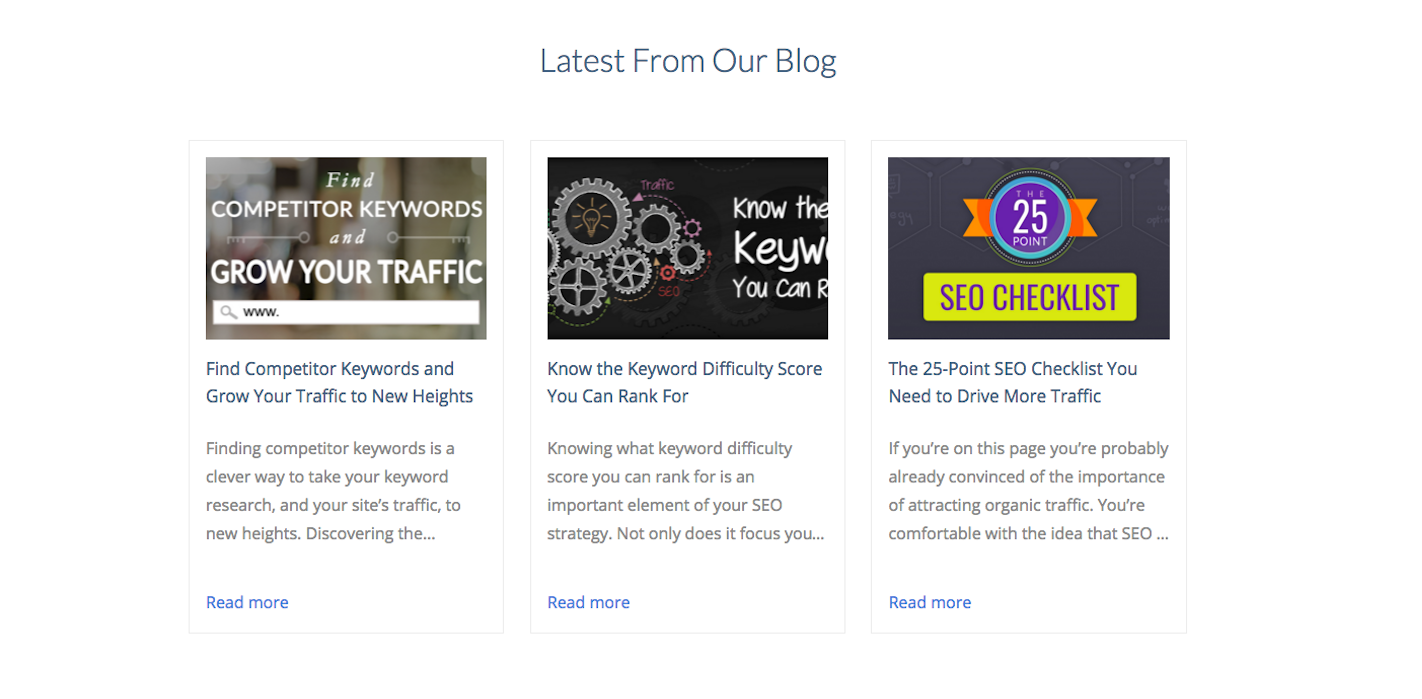
\includegraphics[scale=0.32,keepaspectratio]{{figure/3/when0}.png}
    \caption{Homepage - Asse when}
    \end{figure}
    \FloatBarrier 
Questo tipo di asse informativo non viene presentato in modo immediato e
chiaro, gli articoli non riportano
la data in cui sono stati scritti e quindi non permettono all'utente di capire che 
frequenza di aggionarmento ha il sito. Anche in questo caso le immagini ed
i relativi box contenenti l'articolo non risultano cliccabili, per accedere
all'articolo è necessario cliccare sul titolo dello stesso 
oppure su \quotes{Read more}.\\
Risultato : \textit{5}
\end{flushleft}